\documentclass[a4paper]{article}
\usepackage{geometry}
\usepackage{fontawesome}
\usepackage{titlesec}
\usepackage{enumitem}
\usepackage{xcolor}
\usepackage{hyperref}
\usepackage{graphicx}

% Page settings
\geometry{left=1.8cm,right=1.8cm,top=1cm,bottom=0.5cm}

% Color definitions
\definecolor{mainred}{RGB}{204,0,0}
\definecolor{darkgray}{RGB}{73,73,73}

% Hyperlink settings
\hypersetup{
    colorlinks=true,
    linkcolor=mainred,
    filecolor=mainred,
    urlcolor=darkgray,
}

% Section title format
\titleformat{\section}
{\color{mainred}\Large\bfseries}
{}{0em}{\faGraduationCap\quad}[\titlerule]
\titlespacing{\section}{0pt}{10pt}{6pt}

% Line spacing
\linespread{1.15}

\begin{document}

% Header
\begin{minipage}{0.75\textwidth}
\hspace{-1em}
{\huge\bfseries Qiwei Chen}\medskip

\vspace{0.5em}
\hspace{-0.5em}
\begin{tabular}{@{}l@{\hspace{0.5em}}l@{\hspace{4em}}l@{}}
{\color{darkgray}\faPhone} & +86 131-2312-8852 & {\color{darkgray}\faCalendar} Sep 21, 2003 \\
{\color{darkgray}\faEnvelope} & qiweic10@sjtu.edu.cn & {\color{darkgray}\faUser} CPC Probationary Member \\
{\color{darkgray}\faGithub} & \href{https://github.com/kiwi142857}{\color{darkgray}kiwi142857} & {\color{darkgray}\faHome} \href{https://kiwi142857.github.io/kiwi142857.githhub.io/}{\color{darkgray}Portfolio}
\end{tabular}
\end{minipage}
\begin{minipage}{0.25\textwidth}
\hspace{0.5em}
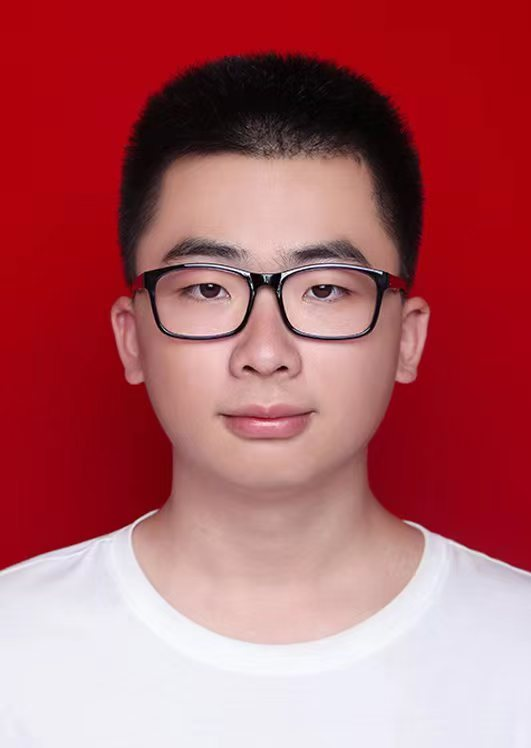
\includegraphics[width=2.8cm]{Kiwi_陈启炜.jpg}
\end{minipage}

\vspace{-2em}
\section*{Education}
\noindent\textbf{\large Shanghai Jiao Tong University} \textbf{Software Engineering} \hfill Sep 2022 - Present\\
\vspace{1em}
\textit{Academic Score: 91.0/100 (Rank: 7/93)} \hfill \textit{GPA: 3.91/4.30 (Rank: 12/93)}\\

\vspace{-1.5em}
\noindent\textbf{Honors}
\begin{itemize}[leftmargin=*,itemsep=0em,topsep=-0.1em]
\item Jiang Scholarship, Outstanding Undergraduate Scholarship \hfill 2023-2024
\item Outstanding Student Leader, SJTU \hfill 2023-2024
\end{itemize}

\section*{Projects}
\begin{itemize}[leftmargin=*,label={},itemsep=0.3em,topsep=0.1em]
\item \textbf{OpenTrustee LLM} \hfill \textit{2024.09 - 2024.11}\\
Led secure LLM deployment on edge devices using OpenTrustee and llama.cpp. Implemented model loading and inference in TEE environment with hardware encryption. Won Third Prize in OpenHarmony National Competition.

\item \textbf{Tiger Language Compiler} \hfill \textit{2024.09 - 2025.01}\\
Developed a compiler with lexical/syntax analysis using Flex/Bison. Implemented semantic analysis, stack frame management, and register allocation. Optimized code generation using LLVM framework.

\item \textbf{CHFS Distributed File System} \hfill \textit{2024.09 - 2025.01}\\
Built GFS-based distributed system with Inode metadata management. Implemented logging, snapshots, and Raft consensus for reliability. Supported concurrent access and fast retrieval for large-scale storage.

\item \textbf{\href{https://base.sjtu.edu.cn/se/Awards.html}{UniGPT Prompt Platform}} \hfill \textit{2024.02 - 2024.09}\\
Led 4-person team in developing microservices-based platform. Implemented k8s orchestration, ELK monitoring, and CI/CD pipeline. Integrated LLM features with langchain4j. Won Excellence Award in Software Exhibition.

\item \textbf{e-BookStore Platform} \hfill \textit{Feb 2024 - Feb 2025}\\
Independently developed a full-stack e-book trading platform. Implemented service discovery and configuration center using Spring Cloud microservices architecture. Utilized Redis for caching and Kafka for service decoupling. Implemented full-text search with ElasticSearch, supporting complex multi-database queries. Deployed using Docker with Nginx load balancing.
\end{itemize}

\section*{Leadership \& Activities}
\begin{minipage}{0.48\textwidth}
\textbf{Student Leadership}
\begin{itemize}[leftmargin=*,itemsep=0.1em,topsep=0.1em]
\item Student Union Member, School of Electronic Information and Electrical Engineering
\item Class Committee Member
\item Member of University Youth League Committee "Si Yuan"
\end{itemize}
\end{minipage}
\begin{minipage}{0.48\textwidth}
\textbf{Social Practice}
\begin{itemize}[leftmargin=*,itemsep=0.1em,topsep=0.1em]
\item Social Research Project in Hunan Province
\item Yue Hongkong and Macao Greater Bay Area Investigation Program
\end{itemize}
\end{minipage}

\section*{Technical Skills}
\begin{itemize}[leftmargin=*,itemsep=0.2em,topsep=0.2em]
\item \textbf{Programming Languages}: Proficient in C/C++; Skilled in Python, Java, JavaScript; Familiar with Swift, Go
\item \textbf{Development Skills}: Microservices Architecture, DevOps, LLM Deployment, Secure Computing, Distributed Systems
\item \textbf{Language Skills}: CET-6 Certification, Strong Technical Documentation Abilities
\end{itemize}

\end{document} 